\section{Códigos e Codificação}

\begin{frame}[allowframebreaks]
  \frametitle{Códigos e Codificação}
  \begin{itemize}
  \item O teorema de Shannon diz que existe uma sequência de códigos tais que:
	se $R < C$, então a probabilidade de erro vai a zero.
  \item Ele não fornece um código ou uma maneira de encontrá-lo.
  \item Codificação típica não é prática, pois haverá formação de blocos com tamanho exponencialmente grandes.
  \item Devemos adicionar redundância suficiente à mensagem para que a mensagem original
	seja decodificada de forma não ambígua.
  \end{itemize}
\end{frame}

\begin{frame}[allowframebreaks]
  \frametitle{Soluções Físicas}
  \begin{itemize}
  \item Podemos estabelecer uma comunicação mais confiável alterando as características físicas
	do meio, reduzindo assim o ruído interferente (diminuir $p$ em um canal binário simétrico).
  \item Utilizar circuitos implementados com componentes de menor tolerância.
  \item Melhorar as condições do ambiente (condições térmicas, poeira e ar).
  \item Utilizar mais área/volume físico por bit.
  \item Utilizar maior potência na transmissão, fazendo que o ruído seja menos significativo. 
  \end{itemize}
\end{frame}

\begin{frame}[allowframebreaks]
  \frametitle{Códigos de Repetição}
  \begin{itemize}
  \item cada símbolo é repetido $k$ vezes
  \item mensagem: $x_1, x_2, \ldots, x_n$
  \item transmitido: $\underbrace{x_1 x_1 \ldots x_1}_{k \text{ vezes}} \underbrace{x_2 x_2 \ldots x_2}_{k \text{ vezes}} \ldots \underbrace{x_n x_n \ldots x_n}_{k \text{ vezes}}$.
  \item Para muitos canais (por exemplo: canal binário simétrico com $p<1/2$), o erro tende a zero quando $k \rightarrow \infty$.
  \item Decodificação simples: quando $k$ é ímpar, utilizar o voto da maioria (que é ótimo para canal binário simétrico).
  \item $R \propto 1/k \rightarrow 0$ quando $k \rightarrow \infty$.
  \item Veja o exemplo apresentado previamente \ref{ex:codrep}.
  \item Estamos supondo que o ruído seja branco, mas algumas vezes o ruído pode ter
	outra característica, como por exemplo um ruído em rajadas. Neste caso,
	o código de repetição seria desastroso. Poderíamos adaptá-lo intercalando 
	os símbolos de forma a minimizar o efeito nocivo de uma rajada.
  \end{itemize}

                \begin{figure}[h!]
                \centering
                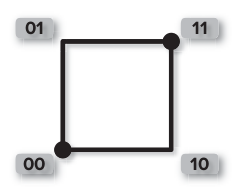
\includegraphics[width=0.4\textwidth]{images/repeatingcode2.png}
		\caption{Código de repetição com $k=2$ ($d_H = 1$).}
                \label{fig:repeatingcode2}
                \end{figure}


                \begin{figure}[h!]
                \centering
                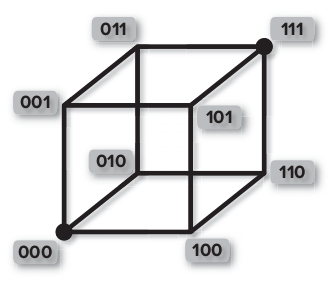
\includegraphics[width=0.4\textwidth]{images/repeatingcode3.png}
		\caption{Código de repetição com $k=3$ ($d_H = 3$).}
                \label{fig:repeatingcode3}
                \end{figure}

	Se $d_H$ (distância de Hamming) for par, podemos detectar $d_H/2$ erros
	e corrigir $d_H/2 - 1$ erros.
	Se $d_H$ for ímpar, podemos corrigir até $(d_H - 1)/2$ erros.
\end{frame}

\begin{frame}[allowframebreaks]
  \frametitle{Código de Verificação de Paridade Simples}
  \begin{itemize}
  \item Entrada/saída binária: $\mathcal{X} = \mathcal{Y} = \{ 0, 1\}$.
  \item Blocos de comprimento $n-1$ bits: $x_{1:n-1}$.
  \item O $n$-ésimo bit é um indicador do número ímpar de bits iguais a $1$ em $x_{1:n-1}$, ou seja,
	\begin{equation}
	x_n \leftarrow \mod \left( \sum_{i=1}^{n-1} x_i , 2 \right) .
	\end{equation}
  \item Uma condição necessária para que uma palavra seja válida é
	\begin{equation}
	\mod \left( \sum_{i=1}^{n} x_i , 2 \right) = 0 .
	\end{equation}
  \item Se ocorrer um número ímpar de erros, esta condição não será satisfeita. Podemos detectar que ocorreu um número ímpar de erros.
  \item Um número par de erros não será detectado.
  \item Só conseguimos detectar alguns erros e não conseguimos corrigir erros.
  \item Verificação de paridade é a base de vários esquemas mais sofisticados de codificação 
	(por exemplo: verificação de paridade de baixa densidade (\textit{low-density parity check}, LDPC),
	código de Hamming, etc.).
  \end{itemize}
\end{frame}



\subsection{Códigos de Hamming}

\begin{frame}[allowframebreaks]
  \frametitle{Código de Hamming $(7,4,3)$}
  \begin{itemize}
  \item comprimento da palavra: $7$; número de bits de informação: $4$; número de bits de verificação de paridade $3$.
  \item $\mathcal{X} = \mathcal{Y} = \{0,1\}$.
  \item $R = 4/7$ bits por utilização do canal.
  \item Bits de dados: $x_0, x_1, x_2, x_3 \in \{0,1\}$.
  \item Bits de redundância: $x_4, x_5, x_6$.
  \item Os bits de paridade são determinados pelas equações:
	\begin{equation}
	x_4 = (x_1 + x_2 + x_3) \mod 2
	\end{equation}
        \begin{equation}
        x_5 = (x_0 + x_2 + x_3) \mod 2
        \end{equation}
        \begin{equation}
        x_6 = (x_0 + x_1 + x_3) \mod 2
        \end{equation}
  \item Exemplo: $(x_0, x_1, x_2, x_3) = (0110)$, então $(x_4,x_5,x_6) = (011)$ e assim a palavra de 7 bits
	será $(0110011)$.
  \item Isto pode ser visto na forma matricial como:
	\begin{equation}
	\mathbf{G} p = x
	\end{equation}
	onde $p$ é o vetor de dados, $p = (x_0, x_1, x_2, x_3)$, e 
	$\mathbf{G}$ é a matriz geradora do código de Hamming e $x$
	os dados com os bits de paridade.
	\begin{equation}
	G = 
        \begin{pmatrix}
	1 & 0 & 0 & 0 \\
	0 & 1 & 0 & 0 \\
	0 & 0 & 1 & 0 \\
	0 & 0 & 0 & 1 \\
	0 & 1 & 1 & 1 \\
	1 & 0 & 1 & 1 \\
	1 & 1 & 0 & 1
	\end{pmatrix}.
	\end{equation}  

  \item Representação gráfica

                \begin{figure}[h!]
                \centering
                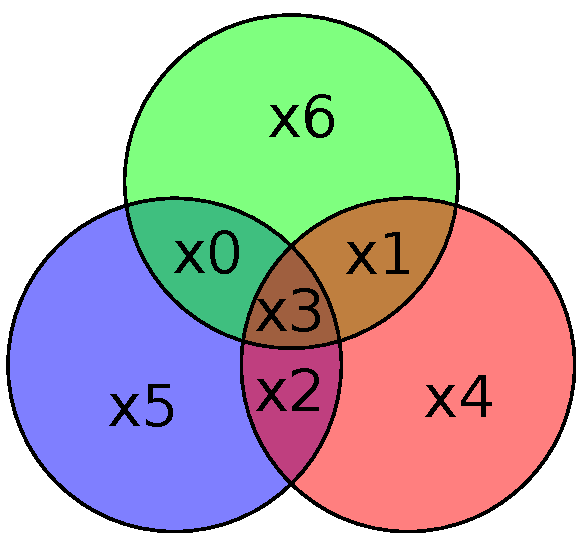
\includegraphics[width=0.4\textwidth]{images/hamming74.pdf}
                \label{fig:hamming74}
                \end{figure}

  \item Podemos também descrever os bits de paridade através das seguintes equações
	\begin{equation}
	\begin{matrix}
	    &   x_1 & + x_2 & + x_3 & + x_4 &       &       & = 0 \\
	x_0 &       & + x_2 & + x_3 &       & + x_5 &       & = 0 \\
	x_0 & + x_1 &       & + x_3 &       &       & + x_6 & = 0 
	\end{matrix}
 	\end{equation}
  \item Alternativamente, podemos escrever $\mathbf{H}x = 0$, onde $x^{T} = (x_0, x_1, \ldots, x_6)$ e
	\begin{equation}
	H = 
	\begin{pmatrix}
	0 & 1 & 1 & 1 & 1 & 0 & 0 \\
	1 & 0 & 1 & 1 & 0 & 1 & 0 \\
	1 & 1 & 0 & 1 & 0 & 0 & 1 
	\end{pmatrix}.
	\end{equation}
  \item As palavras estão no espaço nulo (núcleo)\footnote{
	O núcleo (espaço nulo) de uma transformação linear $L: V \rightarrow W$ entre dois espaços vetoriais é o conjunto
	de todos os elementos de $v \in V$  para os quais $L(v) = 0$, isto é
	\begin{equation}
	\ker(L) = \{ v \in V : L(v) = 0 \},
	\end{equation}
	onde $0$ é o vetor nulo em $W$.
	} de $\mathbf{H}$.
  \end{itemize}  
  \framebreak 
  \begin{itemize}
  \item Note que as colunas de $\mathbf{H}$ são todas as 7 possíveis permutações de colunas de tamanho 3 não-nulas.
  \item As palavras são definidas pelo espaço nulo de $\mathbf{H}$, i.e. $\{x : \mathbf{H}x = 0 , x \neq 0 \}$.
  \item Como o posto\footnote{
	O posto (\textit{rank}) de uma matriz é a dimensão do espaço vetorial gerado pelas colunas da matriz. Isto
	é o mesmo que a dimensão do espaço gerado pelas linhas. O posto é uma medida de `não-degeneração' 
	do sistemas de equações lineares e transformação linear codificada pela matrix.
	} da $\mathbf{H}$ é 3, o espaço nulo será de tamanho 4, visto que $\mathbf{H}$ possui 7 colunas
	\footnote{
	O teorema do posto-nulidade diz que o posto e a nulidade de uma matriz somados devem ser igual ao número de colunas da matriz.
	Se $\mathbf{A}$ é uma matriz $m \times n$, então devemos ter
		\begin{equation}
		\operatorname{rank}(\mathbf{A}) + \operatorname{null}(\mathbf{A}) = n
		\end{equation}
	}. Esperamos assim encontrar $2^4 = 16$ vetores binários neste espaço nulo.
  \end{itemize}
\end{frame}

\begin{frame}[allowframebreaks]
  \frametitle{Código de Hamming $(7,4,3)$}

  \begin{itemize}
  \item 16 vetores no espaço nulo de $\mathbf{H}$:
	\begin{equation}
	\begin{matrix}
	0000000 & 0100101 & 1000011 & 1100110 \\
	0001111 & 0101010 & 1001100 & 1101001 \\ 
	0010110 & 0110011 & 1010101 & 1110000 \\
	0011001 & 0111100 & 1011010 & 1111111
	\end{matrix}
	\end{equation}
  \item Os 4 primeiros bits são os valores variando de 0 a 15 em binário (todas as \textit{strings} binárias de comprimento 4),
	são os bits de dados. Os 3 bits em sequência são os bits de redundância (paridade).
  \item Uma palavra válida do código deve ser um dos vetores acima, $C = \{x : \mathbf{H} x = 0 \}$.
  \item Se $v_1, v_2 \in C$ então $\mathbf{H} (v_1 + v_2) = \mathbf{H} v_1 + \mathbf{H} v_2 = 0$, desta forma,
	$v_1 + v_2 \in C$.
  \item Da mesma forma, $v_1 - v_2 \in C$.
  \item O conjunto de palavras (\textit{codewords}) é um conjunto fechado sob a adição e subtração.
  \item O número mínimo de 1s nestas palavras é 3. Isto é chamado de peso do código. 
	\begin{itemize}
	\item Por que 3? Suponha que o peso do código seja 2 com elementos não nulos nas posições $i$ e $j$.
	Neste caso, por ser uma palavra do código, devemos ter $\mathbf{H} x = 0$, assim a soma 
	da $i$-ésima e $j$-ésima colunas de $\mathbf{H}$ deverá ser igual a zero. Como as colunas de $\mathbf{H}$
	são todas diferentes, a soma de quaisquer duas colunas é não nula. Desta forma não é possível que o código tenha peso 2.
	\item Não podemos ter peso 1 pois as palavras com peso 1 não estão no espaço nulo, pois não existe uma coluna nula em $\mathbf{H}$. 
	\item Peso 3 é possível, pois a soma de duas colunas é igual a uma outra coluna e a soma de dois vetores binários iguais
	é igual a zero ($\mod 2$).
	\end{itemize}
  \item A distância mínima entre palavras deste código também é 3, que é o número mínimo de diferenças entre as palavras.
  	Se $v_1, v_2 \in C = \{ x: \mathbf{H} x = 0 \}$, então $d_H (v_1, v_2) \geq 3$ onde
		\begin{equation}
		d_H(x,y) = \sum_i \mathbf{1}_{\{x(i) \neq y(i)\}}
		\end{equation}
	é a distância de Hamming. Note que, quanto maior a distância entre as palavras de um código, menor a chance
	de haver confusão se a mensagem enviada for corrompida por ruído. É possível assim corrigir erros. I.e.,
	se $\hat{v}$ é uma palavra recebida, então basta adotar a seguinte estratégia de decodificação:
	encontrar $i^\ast = \argmin_i d_H(\hat{v},v_i)$.
                \begin{figure}[h!]
                \centering
                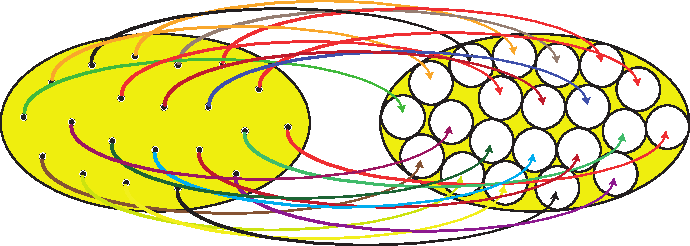
\includegraphics[width=0.5\textwidth]{images/binpack.pdf}
                \label{fig:binpack2}
                \end{figure}
  	Suponha que $v_1, v_2 \in C$ difiram em apenas duas posições. Neste caso, $\mathbf{H} (v_1 - v_2)$
	será a diferença ou soma de duas colunas de $\mathbf{H}$ ($\mod 2$). Como $v_1, v_2 \in C$ 
	teremos $(v_1 - v_2) \in C$. Não poderemos ter a diferença ou soma de quaisquer duas colunas de $\mathbf{H}$
	igual a zero, desta forma $v_1,v_2$ não podem diferir em apenas duas posições.
  \end{itemize}
\end{frame}
\note{
A distância de Hamming entre duas palavras pode ser calculada fazendo um XOR
entre elas e contabilizando o número de uns.

As propriedades de um código de bloco de detectar e corrigir erros dependem
da distância de Hamming mínima entre palavras deste código.
Para detectar $d$ erros de forma confiável, precisamos de uma distância
mínima de $d+1$ entre as palavras do código, número de trocas de bits necessária para
gerar uma outra palavra válida no código. Da mesma forma, para corrigir
$d$ erros, precisamos de uma distância mínima de $2d+1$.
Assumimos o pressuposto de que um maior número de erros é menos provável
e assim corrige-se o erro escolhendo a palavra válida mais próxima 
(menor número de bits trocado).
}
\note{
Seja um código com mensagens de comprimento $n=m+r$, com $m$ bits de dados
e $r$ bits de paridade. Vamos analisar o caso de corrição de um único bit.
Cada palavra possui $n$ vizinhos inválidos e assim $n+1$ padrões associados
a ela ($n$ inválidos e a palavra do código). São $2^m$ palavras no código.
O total de sequências possíveis com $n$ bits é $2^n$. Demos ter então
$(n+1) 2^m \leq 2^n$. Usando $n=m+r$, teremos
\begin{equation}
(m+r+1) \leq 2^r .
\end{equation}
Dado $m$ podemos calcular o número de bits de verificação necessários para
corrigir um único erro.
}


\begin{frame}[allowframebreaks]
  \frametitle{Código de Hamming - Canal Binário Simétrico}

  \begin{itemize}
  \item A decodificação de máxima verosimilhança requer o conhecimento das características do canal
	e ainda é um problema NP-difícil.
  \item Vamos assumir que temos um BSC($p$) (canal binário simétrico com probabilidade de troca $p$).
  \item $x = (x_0, x_1, \ldots, x_6)$ é transmitido, e será recebido
	\begin{equation}
	y = x + z = (x_0 + z_0, x_1 + z_1, \ldots, x_6 + z_6) ,
	\end{equation}
	onde $z = (z_0, z_1, \ldots, z_6)$ é o vetor de ruido aditivo.
  \item Recebemos $y$ e queremos determinar $x$. Iremos calcular a síndrome de $y$
	\begin{equation}
	s = \mathbf{H} y = \mathbf{H} (x+z) = \underbrace{\mathbf{H} x}_{=0} + \mathbf{H} z = \mathbf{H} z
	\end{equation}
  \item Se $s=0$, então todos as verificações de paridade são satisfeitas por $y$, o que é uma condição 
	necessária para que tenhamos uma palavra correta.
  \item $s = \mathbf{H} z$ é uma combinação linear das colunas de $\mathbf{H}$
	\begin{equation}
	s = z_0 \begin{pmatrix} 0 \\ 1 \\ 1 \end{pmatrix} + z_1 \begin{pmatrix} 1 \\ 0 \\ 1 \end{pmatrix} + z_2 \begin{pmatrix} 1 \\ 1 \\ 0 \end{pmatrix} + \ldots + z_6 \begin{pmatrix} 0 \\ 0 \\ 1 \end{pmatrix}
	\end{equation}
  \item Como $y=x+z$, basta encontrar $z$ para determinar $x$, já que $y$ é conhecido.
  \item Precisamos resolver $s = \mathbf{H} z$, um sistema de 3 equações e 7 variáveis. Teremos 4 graus de liberdade.
	Como as variáveis são binárias, teremos $2^{4} = 16$ possíveis soluções.
  \item Exemplo: Suponha que $y^T = 0111001$ seja recebido (não é uma palavra válida), então calcularemos a
	síndrome de $y$, $s = \mathbf{H} y = \mathbf{H} z = (101)^T$ e as 16 possíveis soluções para $z$ são
	\begin{equation}
	\begin{matrix}
	0100000 & 0010011 & 0101111 & 1001001 \\
	1100011 & 0001010 & 1000110 & 1111010 \\
	0000101 & 0111001 & 1110101 & 0011100 \\
	0110110 & 1010000 & 1101100 & 1011111
	\end{matrix}
	\end{equation}
  \item Dentre os 128 possíveis vetores que poderíamos ter, restringimos a apenas 16.
  \item Qual é a probabilidade de cada possível solução? Assumindo que temos um canal binário
	simétrico com $p < 1/2$, a solução mais provável é aquela com menor peso. 
	Qualquer solução com peso $k$ possui probabilidade $p^k$.
  \item Note que existe apenas uma possível solução com peso 1. Esta é a solução mais provável.
  \item A solução mais provável, para o exemplo, é $z = (0100000)^T$ e assim teremos
	$y = x + z$, como $y = (0111001)^T$ teremos a palavra $x = (0011001)^T$, assim os
	bits de informação são $0011$.
  \item Para qualquer $s$, existe uma única solução de peso mínimo para $z$ em $s = \mathbf{H} z$.
  \item Se $s = (000)^T$, então a única solução é $z=(0000000)^T$.
  \item Para uma solução de peso 1, qualquer outro $s$ será igual a uma das colunas de $\mathbf{H}$,
	poderemos assim gerar $z$ fazendo o bit correspondente igual a 1.
  \end{itemize}

\end{frame}

\begin{frame}[allowframebreaks]
  \frametitle{Procedimento de Decodificação de Hamming}

  Procedimento de decodificação de síndrome para um dado $y$ recebido:
  \begin{enumerate}
  \item Calcular a síndrome $s = \mathbf{H} y$.
  \item Se $s = (000)^T$, faça $z \leftarrow (0000000)^T$ e vá ao passo 4.
  \item Caso contrário, localize a única coluna de $\mathbf{H}$ igual a $s$, faça $z$ um vetor cheio de zeros mas
	com 1 na posição correspondente.
  \item Faça $x \leftarrow y+z$
  \item saída: $(x_0, x_1, x_2, x_3)$ 
  \end{enumerate}

  Este procedimento é capaz de corrigir um único bit de erro, mas falha quando há mais do que um único bit de erro.
\end{frame}

\begin{frame}[allowframebreaks]
  \frametitle{Visualização do procedimento de decodificação}
  \begin{itemize}
  \item O procedimento de decodificação pode ser visualizado através de um diagrama de Venn.
                \begin{figure}[h!]
                \centering
                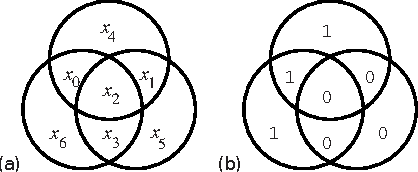
\includegraphics[width=0.5\textwidth]{images/venhamm.pdf}
                \label{fig:venhamm}
                \end{figure}

  \item Os bits de dados ($x_0,x_1,x_2,x_3$) estão nas intersecções e fora delas os bits de paridade ($x_4,x_5,x_6$).
  \item Dentro de cada círculo devemos ter um número par de bits iguais a 1, indicando que não há erro.

 	\begin{equation}
	x_4 \equiv ( x_0 + x_1 + x_2 ) \mod 2
	\end{equation}
        \begin{equation}
        x_5 \equiv ( x_1 + x_2 + x_3 ) \mod 2
        \end{equation}
        \begin{equation}
        x_6 \equiv ( x_0 + x_2 + x_3 ) \mod 2
        \end{equation}
  \item A síndrome pode ser vista como o caso em que a condição de paridade não é satisfeita.
  \item Foi dito que, para $s \neq (0,0,0)$ sempre existe um \textit{flip} de bit que irá fazer com que todas condições de paridade 
	sejam satisfeitas.

                \begin{figure}[h!]
                \centering
                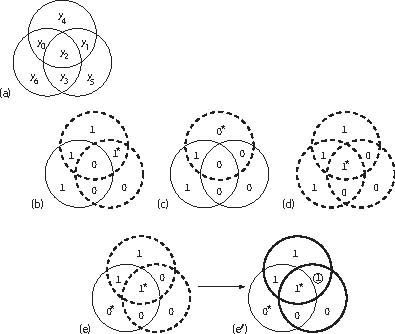
\includegraphics[width=0.65\textwidth]{images/venhamm2.pdf}
                \label{fig:venhamm2}
                \end{figure}

  \item Os bits assinalados com $ ^\ast$ são aqueles com erro. Nos casos (b), (c) e (d) podemos corrigir este erro.
	No caso (e), ao buscar corrigir este erro, introduziremos um novo erro (i.e. introduzindo um novo erro,
	teremos 3 erros, o que corresponde a uma palavra válida no código de Hamming (7,4,3)).
  \end{itemize}
\end{frame}

\begin{frame}[allowframebreaks]
  \frametitle{Codificação}
  \begin{itemize}
  \item Existem outros algoritmos de codificação.
  \item Códigos de Reed Salomon
  \item Códigos de Bose, Ray-Chaudhuri, Hocquenghem
  \item Códigos Convolucionais
  \item Códigos Turbo
  \item Códigos de Verificação de Baixa Densidade
  \item Todos desenvolvidos na busca de obtermos bons códigos com baixa taxa e atingir o limite de Shannon.
  \end{itemize}
\end{frame}




\subsection{Exercícios}
\begin{frame}[allowframebreaks]
  \frametitle{Código Hamming}
  % ~/ee/ufsj/2014_02/ti/aula/bilmes/hw7.pdf
  \begin{exercise}[Código Hamming]
  Utilizando o código de Hamming (7,4,3), realize a decodificação das sequências recebidas abaixo
  utilizando para tanto o procedimento de decodificação de Hamming.

        \begin{equation}
        H = 
        \begin{pmatrix}
        0 & 1 & 1 & 1 & 1 & 0 & 0 \\
        1 & 0 & 1 & 1 & 0 & 1 & 0 \\
        1 & 1 & 0 & 1 & 0 & 0 & 1 
        \end{pmatrix}.
        \end{equation}


  \exercisebreak

  \begin{enumerate}[a)]
  \item $y = 1101011$
  \end{enumerate}
  \textit{(solução)}

  calculando a síndrome teremos
    \begin{align}
    s = \mathbf{H} y =  
	\begin{pmatrix}
        0 & 1 & 1 & 1 & 1 & 0 & 0 \\
        1 & 0 & 1 & 1 & 0 & 1 & 0 \\
        1 & 1 & 0 & 1 & 0 & 0 & 1 
        \end{pmatrix} 
	\begin{pmatrix} 1\\ 1\\ 0\\ 1\\ 0\\ 1\\ 1 \end{pmatrix} &= 
	\begin{pmatrix} 0 \\ 1\\ 0\end{pmatrix} 
    \end{align}

    \exercisebreak

    $s = \mathbf{H} z$ é uma combinação linear das colunas de $\mathbf{H}$

    \begin{equation}
    s = z_0 \begin{pmatrix} 0 \\ 1 \\ 1 \end{pmatrix} + z_1 \begin{pmatrix} 1 \\ 0 \\ 1 \end{pmatrix} + z_2 \begin{pmatrix} 1 \\ 1 \\ 0 \end{pmatrix} + \ldots + z_6 \begin{pmatrix} 0 \\ 0 \\ 1 \end{pmatrix}
    \end{equation}

   
    as 16 possíveis soluções seriam:
        \begin{equation}
        \begin{matrix}
	0101000 & 1011000 & 1100100 & 0010100 \\
	0000010 & 1110010 & 1001110 & 0111110 \\
	1000001 & 0110001 & 0001101 & 1111101 \\
	1101011 & 0011011 & 0100111 & 1010111
        \end{matrix}
        \end{equation}

   \exercisebreak

   vamos escolher aquela com peso 1, basta fazer $z$ um vetor nulo e inserir $1$ apenas 
   na posição correspondente à coluna de $\mathbf{H}$ igual a $s$

  \begin{equation}
  z = (0000010)^T
  \end{equation}

  Assim, iremos decodificar 
  \begin{equation}
  \hat{x} = y + z = 1101011 + 0000010 = 1101001
  \end{equation}

  podemos verificar que $\mathbf{H}x = 0$
  
  \exercisebreak

  \begin{enumerate}[b)]
  \item $y = 0110110$
  \end{enumerate}

  \textit{(solução)}

  síndrome $s = (1 0 1)^T$

  $z = 0100000$ 
 
  \begin{equation}
  \hat{x} = y + z = 0110110 + 0100000 = 0010110
  \end{equation}


  \end{exercise}
\end{frame}


\subsection{Código de Hamming Estendido}
\begin{frame}[allowframebreaks]
  \frametitle{Código de Hamming Estendido}

  O Código de Hamming $(7,4,3)$ pode ser facilmente estendido 
  para o código $(8,4,4)$, bastando para tanto, acrescentar um 
  bit de paridade extra conforme a Figura \ref{fig:hamming84}.

                \begin{figure}[h!]
                \centering
                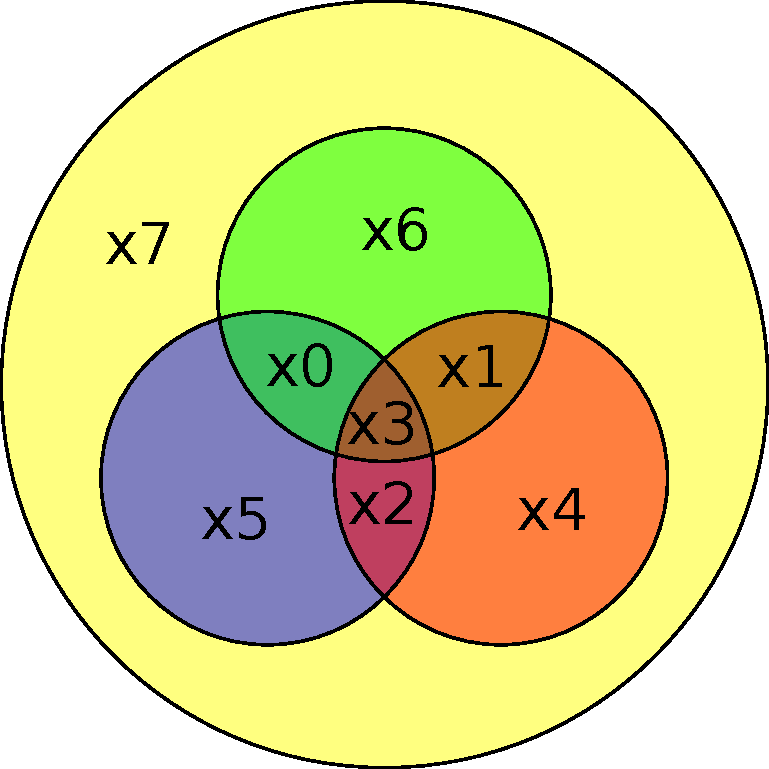
\includegraphics[width=0.4\textwidth]{images/hamming84.pdf}
                \label{fig:hamming84}
                \end{figure}

  \begin{itemize}
    \item Bits de dados: $x_0, x_1, x_2, x_3 \in \{0,1\}$.
    \item Bits de paridade: $x_4, x_5, x_6, x_7 \in \{0,1\}$.
    \item Os bits de paridade são determinados pelas equações:
        \begin{equation}
        x_4 = (x_1 + x_2 + x_3) \mod 2
        \end{equation}
        \begin{equation}
        x_5 = (x_0 + x_2 + x_3) \mod 2
        \end{equation}
        \begin{equation}
        x_6 = (x_0 + x_1 + x_3) \mod 2
        \end{equation}
	\begin{eqnarray}
	x_7 &=& (x_0 + x_1 + x_2 + x_3 + x_4 + x_5 + x_6) \mod 2 \\
	    &=& (3 x_0 + 3 x_1 + 3 x_2 + 4 x_3 ) \mod 2 \\
	    &=& (x_0 + x_1 + x_2) \mod 2
	\end{eqnarray}	
    \item A matriz geradora será
        \begin{equation}
        G = 
        \begin{pmatrix}
        1 & 0 & 0 & 0 \\
        0 & 1 & 0 & 0 \\
        0 & 0 & 1 & 0 \\
        0 & 0 & 0 & 1 \\
        0 & 1 & 1 & 1 \\
        1 & 0 & 1 & 1 \\
        1 & 1 & 0 & 1 \\ \hdashline[2pt/2pt]
	1 & 1 & 1 & 0
        \end{pmatrix}.
        \end{equation}

    \item A matriz de verificação de paridade será
        \begin{equation}\label{eq-Hmat844}
        H = 
        \left(
        \begin{array}{ccccccc;{2pt/2pt}c}
        0 & 1 & 1 & 1 & 1 & 0 & 0 & 0 \\
        1 & 0 & 1 & 1 & 0 & 1 & 0 & 0 \\
        1 & 1 & 0 & 1 & 0 & 0 & 1 & 0 \\ \hdashline[2pt/2pt]
        1 & 1 & 1 & 1 & 1 & 1 & 1 & 1
        \end{array}
        \right),
        \end{equation} 

       ou, de forma equivalente,

        \begin{equation}
        H = 
        \left(
        \begin{array}{ccccccc;{2pt/2pt}c}
        0 & 1 & 1 & 1 & 1 & 0 & 0 & 0 \\
        1 & 0 & 1 & 1 & 0 & 1 & 0 & 0 \\
        1 & 1 & 0 & 1 & 0 & 0 & 1 & 0 \\ \hdashline[2pt/2pt]
        1 & 1 & 1 & 0 & 0 & 0 & 0 & 1
        \end{array}
        \right).
        \end{equation}


     \item A distância mínima do código de Hamming estendido $(8,4,4)$ é de 4. 
	O código de Hamming $(7,4,3)$ possui distância mínima de 3.

    \item O número mínimo de 1s nas palavras no código de Hamming estendido $(8,4,4)$ é 4. 
	Ou seja, o peso do código é 4. (Iremos verificar para a matriz dada na Equação \ref{eq-Hmat844})
        \begin{itemize}
	\item Não podemos ter peso 1 pois as palavras com peso 1 não estão no espaço nulo de 
	$\mathbf{H}$. Suponha que a palavra $x$ seja não nula apenas na posição $i$. Então
	$\mathbf{H} x$ será igual à $i$-ésima coluna de $\mathbf{H}$. Mas não existe coluna 
	nula em $\mathbf{H}$, desta forma não é possível ter $\mathbf{H} x = 0$ com palavras
	de peso 1.
        \item Suponha que o peso do código seja 2, com elementos não nulos nas posições $i$ e $j$.
        Neste caso, por ser uma palavra do código, devemos ter $\mathbf{H} x = 0$, assim a soma
        da $i$-ésima e $j$-ésima colunas de $\mathbf{H}$ deverá ser igual a zero. 
	Como as colunas de $\mathbf{H}$ são todas diferentes, a soma de quaisquer duas colunas é 
	não nula. Desta forma não é possível que o código tenha peso 2.
        \item Peso 3 também não é possível. Note que a última linha de $\mathbf{H}$ é toda igual a 1,
	logo ao somar 3 colunas de $\mathbf{H}$, no último índice estaremos somando 1 três vezes, e
	terá como resultado 1. Desta forma, será impossível obter como resultado o $0$ desejado.
	\item Peso 4 será possível.
        \end{itemize}


     \item A distância mínima entre palavras em $C$ é 4.
	\begin{itemize} 
	\item Suponha que $v_1, v_2 \in C$ difiram em apenas uma posição. Sabemos que $C$ é fechado
	em relação à soma, logo $(v_1 - v_2) \in C$. Como $v_1, v_2$ se diferem em apenas uma posição, 
	$\mathbf{H} (v_1 - v_2)$ deverá ser uma coluna de $\mathbf{H}$, mas sabemos que não exite coluna
	de $\mathbf{H}$ nula. Não podemos ter $v_1, v_2$ diferindo em apenas uma posição.
	\item Suponha que $v_1, v_2 \in C$ difiram em apenas duas posições. Neste caso, $\mathbf{H} (v_1 - v_2)$
	será a diferença ou soma de duas colunas de $\mathbf{H}$.  Como $v_1, v_2 \in C$
	teremos $(v_1 - v_2) \in C$. Não poderemos ter a diferença ou soma de quaisquer duas colunas de $\mathbf{H}$
	igual a zero, desta forma $v_1,v_2$ não podem diferir em apenas duas posições.
	\item Suponha que $v_1, v_2 \in C$ difiram em apenas três posições. Mais uma vez chegaremos 
	em contradição, pois teremos a diferença ou soma de quaisquer três colunas de $\mathbf{H}$,
	que não poderá ser igual a zero devido à última linha de $\mathbf{H}$ ser toda igual a 1.
	\end{itemize}



  \item Procedimento de decodificação de síndrome para um dado $y$ recebido:
  \begin{enumerate}
  \item Calcular a síndrome $s = \mathbf{H} y$.
  \item Se $s = (000)^T$, faça $z \leftarrow (00000000)^T$ e vá ao passo 4.
  \item Caso contrário, localize a única coluna de $\mathbf{H}$ igual a $s$, faça $z$ um vetor cheio de zeros mas
        com 1 na posição correspondente.
  \item Faça $x \leftarrow y+z$
  \item saída: $(x_0, x_1, x_2, x_3)$
  \end{enumerate}
  \item O procedimento é o mesmo utilizado no código do Hamming $(7,4,3)$.
  \item Este procedimento é capaz de corrigir um único bit de erro e detectar dois erros, 
	mas falha quando mais do que dois bits são trocados (bits de erro).
\end{itemize}

\end{frame}



\subsection{Algoritmo do Código de Hamming}
\begin{frame}[allowframebreaks]
  \frametitle{Algoritmo do Código de Hamming}


\adjustbox{max height=\dimexpr\textheight-5.5cm\relax,
           max width=\textwidth}{

\begin{tabular}{|*{22}{c|}}
  \multicolumn{2}{ c }{ \ }  & \rot{1} & \rot{10} & \rot{11} & \rot{100} & \rot{101} & \rot{110} & \rot{111} & \rot{1000} & \rot{1001} & \rot{1010} & \rot{1011} & \rot{1100} & \rot{1101} & \rot{1110} & \rot{1111} & \rot{10000} & \rot{10001} & \rot{10010} & \rot{10011} & \rot{10100} \\
  \hline
  \multicolumn{2}{ |c| }{posição do bit} & 1 & 2 & 3 & 4 & 5 & 6 & 7 & 8 & 9 & 10 & 11 & 12 & 13 & 14 & 15 & 16 & 17 & 18 & 19 & 20 \\  \hline 
  \multicolumn{2}{ |c| }{bits de dado codificados} & \cellcolor{blue!25} $p_1$ & \cellcolor{red!25} $p_2$ & $p_3$ & \cellcolor{green!25} $p_4$ & $p_5$ & $p_6$ & $p_7$ & \cellcolor{yellow!25} $p_8$ & $p_9$ & $p_{10}$ & $p_{11}$ & $p_{12}$ & $p_{13}$ & $p_{14}$ & $p_{15}$ & \cellcolor{orange!25} $p_{16}$ & $p_{17}$ & $p_{18}$ & $p_{19}$ & $p_{20}$ \\  \hline 
  \multirow{5}{*}{\rotatebox[origin=c]{90}{ \parbox[c]{5em}{Cobertura dos bits de paridade}}} 
  	& \cellcolor{blue!25} $p_1$ & 		X &   & X &   & X &   & X &   & X &   & X &   & X &   & X &   & X &   & X & \\ \cline{2-22}
  	& \cellcolor{red!25} $p_2$ & 		  & X & X &   &   & X & X &   &   & X & X &   &   & X & X &   &      & X & X &  \\ \cline{2-22} 
  	& \cellcolor{green!25} $p_4$ & 		  &   &   & X & X & X & X &   &   &   &   & X & X & X & X &   &   &   &   &  X \\ \cline{2-22}
  	& \cellcolor{yellow!25} $p_8$ & 		  &   &   &   &   &   &   & X & X & X & X & X & X & X & X &   &  &   &   &   \\ \cline{2-22}
  	& \cellcolor{orange!25} $p_{16}$ & 	  &   &   &   &   &   &   &   &   &   &   &   &   &   &   & X & X & X  & X & X \\
  \hline
\end{tabular}

}



\begin{itemize}
\item $p_1$: o primeiro bit de paridade abarcará as posições em que sua representação
	na forma binária apresenta o bit 1 em seu primeiro bit, ou seja, a posição menos significativa.
	São elas: 1 (\textbf{1}), 3 (1\textbf{1}), 5 (10\textbf{1}), 7 (11\textbf{1}), 9 (100\textbf{1}),
	11 (101\textbf{1}), etc.
\item $p_2$: o segundo bit de paridade abarcará as posições em que sua representação
        na forma binária apresenta o bit 1 em seu segundo bit, ou seja, a segundo posição menos significativa.
	São elas: 2 (\textbf{1}0), 3 (\textbf{1}1), 6 (1\textbf{1}0), 7 (1\textbf{1}1), 10 (10\textbf{1}0),
	11 (10\textbf{1}1), etc.
\item $p_3$: o terceiro bit de paridade abarcará as posições em que sua representação
        na forma binária apresenta o bit 1 em seu terceiro bit, ou seja, a terceira posição menos significativa.
	São elas: 4 (\textbf{1}00), 5 (\textbf{1}01), 6 (\textbf{1}10), 7 (\textbf{1}11), 12 (1\textbf{1}00),
	13 (1\textbf{1}01), 14 (1\textbf{1}10), 15 (1\textbf{1}11), etc.
\item e assim por diante...
\end{itemize}

Se utilizarmos $m$ bits de paridade, poderemos realizar a verificação dos bits de 1 a $2^m - 1$.
Subtraindo os bits de paridade, teremos $2^m - 1 - m$ bits que poderão ser utilizados para dados.
Variando $m$, teremos os seguintes códigos de Hamming:

\adjustbox{max height=\dimexpr\textheight-5.5cm\relax,
           max width=\textwidth}{
\begin{tabular}{lllll}
bits de paridade & total de bits & bits de dados & nome & taxa \\ \hline
2 & 3  & 1  & Hamming(3,1)	& $1/3 \approx 0.333$ 	\\ \hline
3 & 7  & 4  & Hamming(7,4)	& $4/7 \approx 0.571$	\\ \hline
4 & 15 & 11 & Hamming(15,11)	& $11/15 \approx 0.733$	\\ \hline
5 & 31 & 26 & Hamming(31,26) 	& $26/31 \approx 0.839$	\\ \hline
\end{tabular}
}

\end{frame}



\begin{frame}[allowframebreaks]
    Utilizamos anteriormente a seguinte formulação:
        $x^{T} = (x_0, x_1, \ldots, x_6)$ e
        \begin{equation}
        H = 
        \begin{pmatrix}
        0 & 1 & 1 & 1 & 1 & 0 & 0 \\
        1 & 0 & 1 & 1 & 0 & 1 & 0 \\
        1 & 1 & 0 & 1 & 0 & 0 & 1 
        \end{pmatrix}.
        \end{equation}

      Podemos trocar o ordenamento dos bits, sem prejuízo algum, e desta forma deveremos também
      trocar o ordenamento das colunas da matriz $\mathbf{H}$.

      Suponha que seja feita a seguinte permutação
      $(x_0, x_1, \ldots, x_6) \rightarrow (x_4, x_2, x_3, x_0, x_1, x_5, x_6)$. 
      A nova matriz $\mathbf{H}$ será dada então por
        \begin{equation}
        H = 
        \begin{pmatrix}
        1 & 1 & 1 & 0 & 1 & 0 & 0 \\
        0 & 1 & 1 & 1 & 0 & 1 & 0 \\
        0 & 0 & 1 & 1 & 1 & 0 & 1 
        \end{pmatrix}.
        \end{equation}


    A soma de quais quer duas equações de restrição de paridade fornece uma nova equação.
    Por exemplo, se somarmos as equações representadas pela 1a e 2a linha, teremos
    \begin{equation}
    x_4 + 2 x_2 + 2 x_3 + x_0 + x_1 + x_5 = x_4 + x_0 + x_1 + x_5 ,
    \end{equation}
    que é uma nova equação equação de verificação de paridade, a qual poderemos adicionar à matriz $\mathbf{H}$:
        \begin{equation}
        H' = 
        \begin{pmatrix}
        1 & 1 & 1 & 0 & 1 & 0 & 0 \\
        0 & 1 & 1 & 1 & 0 & 1 & 0 \\
        0 & 0 & 1 & 1 & 1 & 0 & 1 \\
	1 & 0 & 0 & 1 & 1 & 1 & 0
        \end{pmatrix}.
        \end{equation}
    Note que a quarta linha é a soma (módulo 2) das linhas 1 e 2. Note ainda que todas as linhas são
    deslocamentos cíclicos de uma outra linha. Podemos ainda descartar uma das verificações de paridade
    redundante, descartando, por exemplo, a primeira linha, obtendo
        \begin{equation}
        H'' = 
        \begin{pmatrix}
        0 & 1 & 1 & 1 & 0 & 1 & 0 \\
        0 & 0 & 1 & 1 & 1 & 0 & 1 \\
        1 & 0 & 0 & 1 & 1 & 1 & 0
        \end{pmatrix}.
        \end{equation}

     Realizando o mesmo procedimento acima para gerar as equações de paridade redundantes, podemos obter uma
     matriz super-redundante com sete linhas de verificação de paridade:
        \begin{equation}
        H' = 
        \begin{pmatrix}
        1 & 1 & 1 & 0 & 1 & 0 & 0 \\
        0 & 1 & 1 & 1 & 0 & 1 & 0 \\
        0 & 0 & 1 & 1 & 1 & 0 & 1 \\
        1 & 0 & 0 & 1 & 1 & 1 & 0 \\
	0 & 1 & 0 & 0 & 1 & 1 & 1 \\
	1 & 0 & 1 & 0 & 0 & 1 & 1 \\
	1 & 1 & 0 & 1 & 0 & 0 & 1
        \end{pmatrix}.
        \end{equation}

     Esta matriz é uma matriz cíclica, em que cada linha é uma permutação cíclica da primeira linha.
     \textit{Códigos Cíclicos} são códigos que utilizam uma matriz cíclica para verificação de paridade.
     As palavras de código de tais códigos também possuem a propriedade de serem cíclicos, ou seja,
     qualquer permutação cíclica de uma palavra de código é também uma palavra de código.
\end{frame}
